\documentclass{article}
\usepackage{multicol}
\usepackage{listings}
\usepackage[margin=1.25in]{geometry}
\usepackage{graphicx}
\usepackage{float}
\usepackage{subcaption}
\newcommand*{\Scale}[2][4]{\scalebox{#1}{$#2$}}%
\newcommand*{\Resize}[2]{\resizebox{#1}{!}{$#2$}}%
\graphicspath{ {./Figures/} }

\title{Lab report}
\date{2019-03-13}
\author{Mark Kent}

\begin{document}

\section{Objectives}

\indent
The objective for this lab was to build a qunatizer for PCM and creating a Delta
modulator in MATLAB. The secondary objective is to understnad how to quantiy the
the quantization noise of a PCM signal and the granulation noise of a delta
modulated signal.


\section{Procedure}
The MATLAB code that was used in the lab is found in Appendix A. Supplemntary function are found in Appendix B
\subsection{PCM}

We began defining a signal that will be Pulse Code Modulated.
The signal that was used was defined as:

\begin{center}
$
y(t) = sin(2 \pi t) + sin(4 \pi t) +sin(5 \pi t) +sin(9 \pi t) +sin(10 \pi t) +sin(24 \pi t)
$
\end{center}

\noindent
The time interval was from 0 to 1 with a time step of 0.001.\\ \\
\noindent
The signal was quantized using the custom function quantized sample.
The variable quantized data holds integer values that represent the level of the signal.
These values would normally be encoded into a binary stream and then transmitted but
for the purpose of this lab that wouldn't be necessary.
\noindent
The resulting data was reconstructed using the custom function reconstructed data.

\subsection{Delta Modulation}

The signal that was used for this portion of the lab was defined as:\\
\begin{center}
\large
$
e^{-2 t^2}cos(\pi t)
$
\normalsize
\end{center}
\noindent
with a time interval from -3 to 3 with a time step of 0.01.\\ \\
\noindent
The optimal step size was calculated using:

\begin{center}
\Large
$
E = \frac{\dot{m}(t)\omega}{f_s}
$
\normalsize
\end{center}
\section{Results}
\subsection{PCM}
The following figures are the results of the MATLAB code.
% Figures for 4 Levels
\begin{figure}[H]
  \begin{center}
    \begin{subfigure}[b]{0.4\linewidth}
      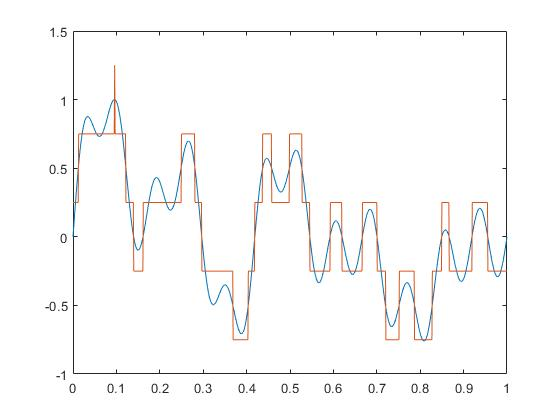
\includegraphics[width = \linewidth]{PCM_4.jpg}
      \caption{Reconstructed signal}
    \end{subfigure}
    \begin{subfigure}[b]{0.4\linewidth}
      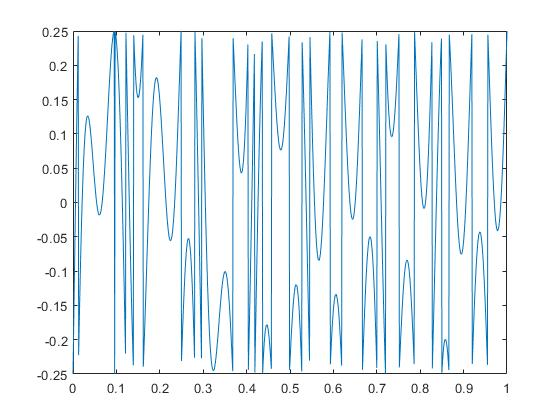
\includegraphics[width = \linewidth]{PCM_4_Error.jpg}
      \caption{Quantization Error}
    \end{subfigure}
    \caption{Signal Quantized with 4 Levels}
    \label{fig:figure1}
  \end{center}
\end{figure}
% Figures for 16 levels
\begin{figure}[H]
  \begin{center}
    \begin{subfigure}[b]{0.4\linewidth}
      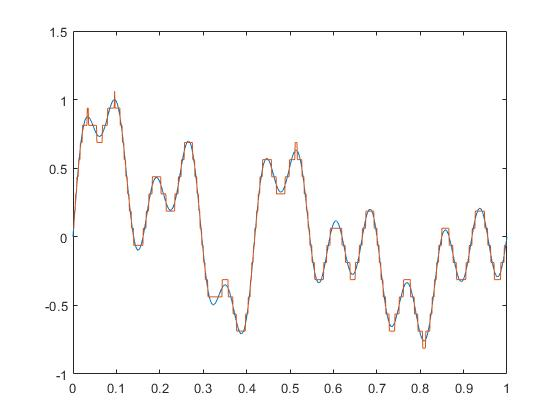
\includegraphics[width = \linewidth]{PCM_16.jpg}
      \caption{Reconstructed signal}
    \end{subfigure}
    \begin{subfigure}[b]{0.4\linewidth}
      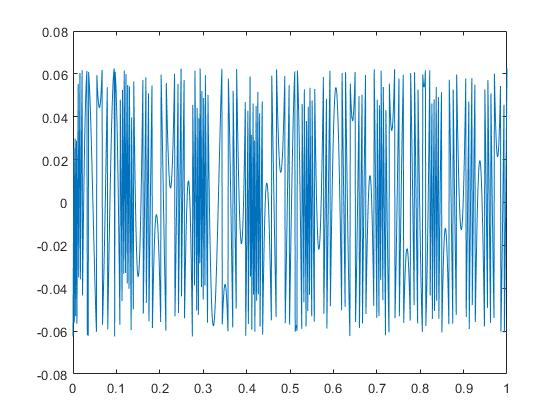
\includegraphics[width = \linewidth]{PCM_16_Error.jpg}
      \caption{Quantization Error}
    \end{subfigure}
    \caption{Signal Quantized with 16 Levels}
    \label{fig:figure2}
  \end{center}
\end{figure}
\noindent
The equation used to calculate the theoretical error is:
\Large
% Theoretical Error Equation
\begin{center}
$ \epsilon = \frac{\hat{m}(t)^2}{3L}$
\end{center}
\normalsize
\noindent
The theoretical error that was calcualted for a normalized, quantized signal with 4 levels was 0.0208.\\
The measured error was found to be 0.0205\\
The theoretical error that was calculated for a normalized, quantized signal with 16 levels was 0.0013\\
The measured error was found to be 0.0013\\
\subsection{Delta Modulation}
The following figures are the results from the Delta Modulation portion of the label
\begin{figure}[H]
  \begin{center}
    \begin{subfigure}[b]{0.4\linewidth}
      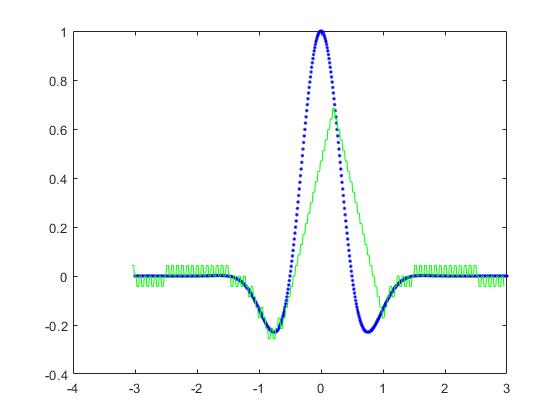
\includegraphics[width = \linewidth]{Del_0_5.jpg}
      \caption{Reconstructed signal}
    \end{subfigure}
    \begin{subfigure}[b]{0.4\linewidth}
      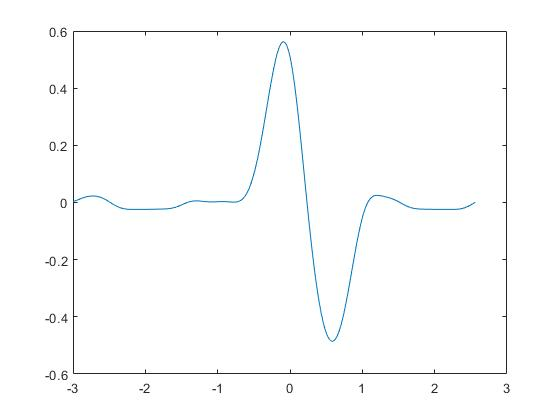
\includegraphics[width = \linewidth]{Del_Error_0_5.jpg}
      \caption{Granulation Error}
    \end{subfigure}
    \caption{Signal Sampled with $E = 0.5 E_0$ Levels}
    \label{fig:figure3}
  \end{center}
\end{figure}
\begin{figure}[H]
  \begin{center}
    \begin{subfigure}[b]{0.4\linewidth}
      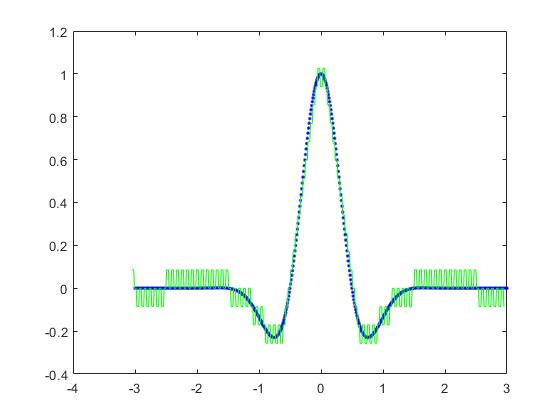
\includegraphics[width = \linewidth]{Del_1.jpg}
      \caption{Reconstructed signal}
    \end{subfigure}
    \begin{subfigure}[b]{0.4\linewidth}
      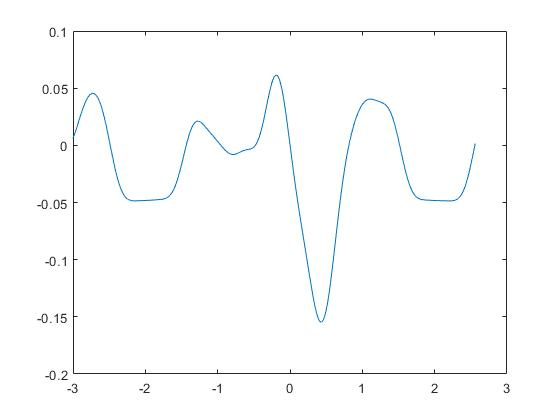
\includegraphics[width = \linewidth]{Del_Error_1.jpg}
      \caption{Granulation Error}
    \end{subfigure}
    \caption{Signal Sampled with $E = E_0$ Levels}
    \label{fig:figure4}
  \end{center}
\end{figure}
\begin{figure}[H]
  \begin{center}
    \begin{subfigure}[b]{0.4\linewidth}
      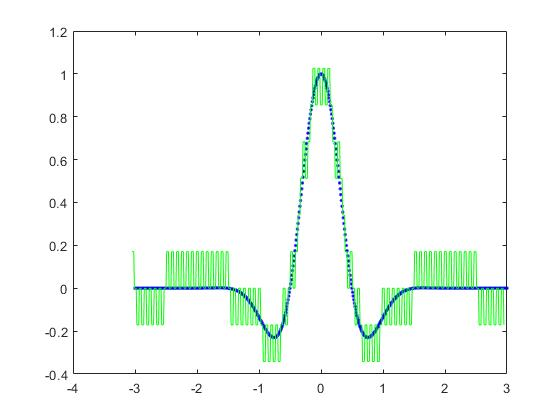
\includegraphics[width = \linewidth]{Del_2.jpg}
      \caption{Reconstructed signal}
    \end{subfigure}
    \begin{subfigure}[b]{0.4\linewidth}
      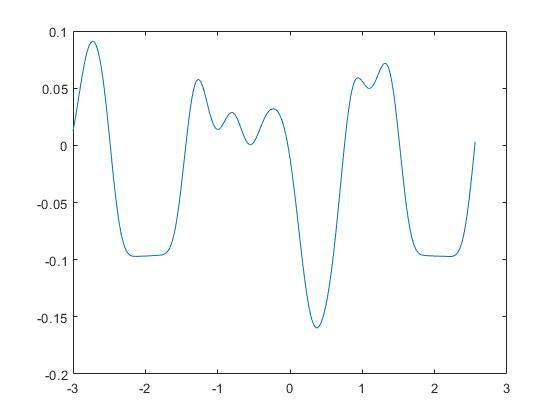
\includegraphics[width = \linewidth]{Del_Error_2.jpg}
      \caption{Granulation Error}
    \end{subfigure}
    \caption{Signal Sampled with $E = 2 E_0$ Levels}
    \label{fig:figure5}
  \end{center}
\end{figure}
\appendix
\section{MATLAB Code}
\begin{lstlisting}[language = MATLAB]
t = 0:0.001:1;
fs = 1000;
L = 4;
signal = sin(t* 2 * pi) + sin(t* 4 * pi) + sin(t* 5 * pi)...
         + sin(t* 9 * pi) + sin(t* 10 * pi) + sin(t* 24 * pi);
signal = signal/max(abs(signal));
quantizedData = quantizedSample(signal, L);

reconstructedData = reconstructQuantized(max(abs(signal)),...
                    L, quantizedData);

plot(t,signal, t, reconstructedData);

q = signal - reconstructedData;
theoreticalError = max(abs(signal)).^2/(3*L^2)
measuredError = mean(q.^2)
var(q)
plot(t, q);

fs= 100*10;
t = -3:1/fs:3;
signal = exp(-2*t.^2).*cos(pi*t);

sampleRatio = 4;

optimalStepSize = pi * max(myDerivative(signal,1/fs))*max(signal)/fs;

[delSignal,estime] = delQuantization(optimalStepSize, signal, fs,...
                     fs/sampleRatio);
recon1 = cumulativeSum(delSignal);
resampled = upsample(delSignal,sampleRatio);

resampled = cumulativeSum(resampled * optimalStepSize);

test1 = cumulativeSum(delSignal * optimalStepSize);
test2 = cumulativeSum(delSignal) * optimalStepSize;
resampled = resampled(1:length(t));
plot(t, signal,'b.', t - 5/fs, resampled,'g');

filtered = filter(DelFilter(fs),[1],resampled);
offset = 44;
plot(t, signal,'b.',t(1:end-offset), filtered(1+offset:end),'g');

shift = 44;
granError = signal(1:end-shift) - filtered(1 + shift:end);
plot(t(1:end - shift),granError);

\end{lstlisting}
\section{Suplementary Code}
\subsection{quantizedSample}
\begin{lstlisting}[language = MATLAB]
function data = quantizedSample(data, numSamples)
maxValue = max(data)*2;
data = data * numSamples / maxValue;
data = floor(data);
end
\end{lstlisting}
\subsection{reconstructQuantized}
\begin{lstlisting}[language = MATLAB]
function data = reconstructQuantized(maxValue, numbLevels, data)
    levelValue = maxValue * 2 / numbLevels;
    data = data*levelValue + levelValue / 2;
end
\end{lstlisting}
\subsection{myDerivative}
\begin{lstlisting}[language = MATLAB]
function dataout = myDerivative(dataIn, samplePeriod);
dataout = (dataIn(2:end) - dataIn(1:end-1))/samplePeriod;
end
\end{lstlisting}
\subsection{delQuantization}
\begin{lstlisting}[language = MATLAB]
function [data,value] = delQuantization(stepSize, signal,...
         signalSampleRate, newSampleRate)

    signal = downsample(signal, ceil(signalSampleRate..
             /newSampleRate));
    data = zeros(1,length(signal));
    error = zeros(1,length(signal));
    value = zeros(1,length(signal));
    data(1) = 1;
    value(1) = stepSize;
    for i = 2:length(signal)
        error(i) = signal(i-1) - value(i-1);
        if(error(i) > 0)
           data(i) = 1;
        else
           data(i) = -1;
        end
        value(i) = value(i-1) + data(i) * stepSize;
    end
end
\end{lstlisting}
\subsection{cumulativeSum}
\begin{lstlisting}[language = MATLAB]
function dataOut = cumulativeSum(dataIn)
    dataOut = zeros(1,length(dataIn));
    dataOut(1) = dataIn(1);
    for i = 2:length(dataIn)
       dataOut(i) = dataOut(i-1) + dataIn(i);
    end
end
\end{lstlisting}
\subsection{DelFilter}
\begin{lstlisting}[language = MATLAB]
function H = DelFilter(Fs)
%DELFILTER Returns a discrete-time filter object.

% MATLAB Code
% Generated by MATLAB(R) 9.4 and Signal Processing Toolbox 8.0.
% Generated on: 06-Mar-2019 20:53:25

% Equiripple Lowpass filter designed using the FIRPM function.

% All frequency values are in Hz.
%Fs = 100;  % Sampling Frequency

Fpass = 1;               % Passband Frequency
Fstop = 4;               % Stopband Frequency
Dpass = 0.057501127785;  % Passband Ripple
Dstop = 0.0001;          % Stopband Attenuation
dens  = 20;              % Density Factor

% Calculate the order from the parameters using FIRPMORD.
[N, Fo, Ao, W] = firpmord([Fpass, Fstop]/(Fs/2), [1 0], [Dpass, Dstop]);

% Calculate the coefficients using the FIRPM function.
b  = firpm(N, Fo, Ao, W, {dens});
Hd = dfilt.dffir(b);
H = Hd.Numerator;
% [EOF]
\end{lstlisting}
\end{document}
